%%%%%%%%%%%%%%%%%%%%%%%%%%%%%%%%%%%%%%%%%
% LaTeX Template
% http://www.LaTeXTemplates.com
%
% Original author:
% Linux and Unix Users Group at Virginia Tech Wiki 
% (https://vtluug.org/wiki/Example_LaTeX_chem_lab_report)
%
% License:
% CC BY-NC-SA 3.0 (http://creativecommons.org/licenses/by-nc-sa/3.0/)
%
%%%%%%%%%%%%%%%%%%%%%%%%%%%%%%%%%%%%%%%%%

%----------------------------------------------------------------------------------------
%	PACKAGES AND DOCUMENT CONFIGURATIONS
%----------------------------------------------------------------------------------------

\documentclass[12pt]{article}
\usepackage{geometry} % Pour passer au format A4
\geometry{hmargin=1cm, vmargin=1cm} % 

\usepackage{graphicx} % Required for including pictures
\usepackage{float} % 

%Français
\usepackage[T1]{fontenc} 
\usepackage[english,francais]{babel}
\usepackage[utf8]{inputenc}
\usepackage{eurosym}
\usepackage{lmodern}
\usepackage{url}
\usepackage{multicol}

%Maths
\usepackage{amsmath,amsfonts,amssymb,amsthm}
%\usepackage[linesnumbered, ruled, vlined]{algorithm2e}
%\SetAlFnt{\small\sffamily}

%Autres
\linespread{1} % Line spacing
\setlength\parindent{0pt} % Removes all indentation from paragraphs

\renewcommand{\labelenumi}{\alph{enumi}.} % 
\pagestyle{empty}
%----------------------------------------------------------------------------------------
%	DOCUMENT INFORMATION
%----------------------------------------------------------------------------------------
\begin{document}

%\maketitle % Insert the title, author and date

% Exercice 1 
\subsection*{Exercice 1} 
Le schéma ci-dessous permet de visualiser une manière de récupérer l’eau de pluie.

\begin{multicols}{2}

  \begin{figure}[H]
    \centering
    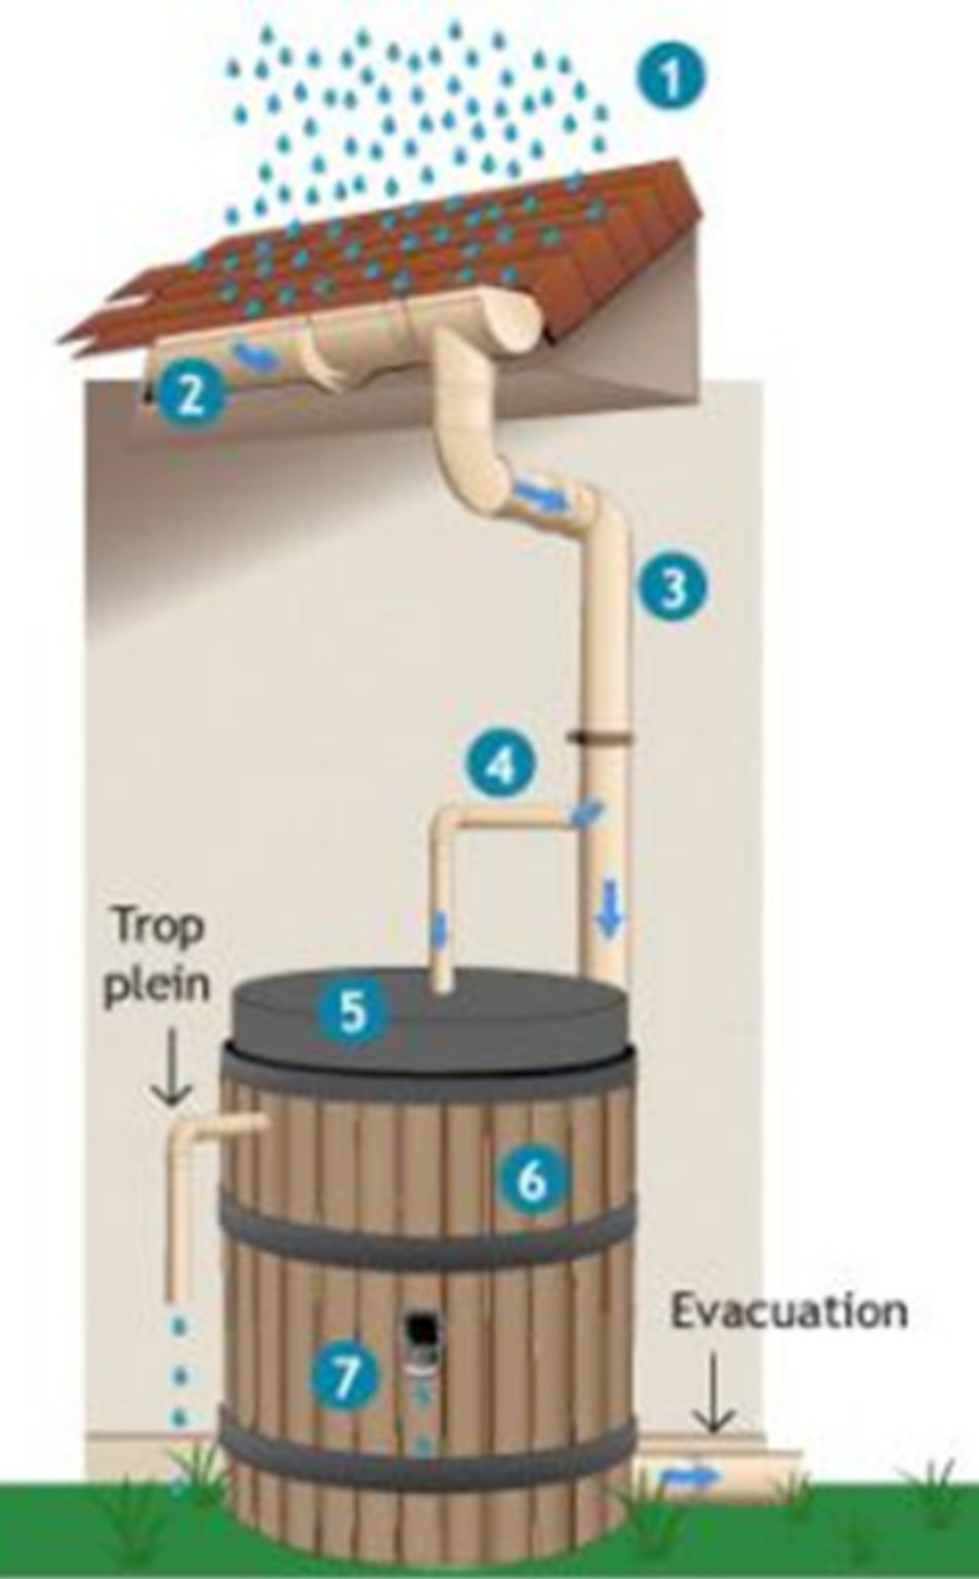
\includegraphics[width=0.8\linewidth]{sources/plan.pdf}
  \end{figure}

\begin{enumerate}
\item[1.] L’eau de pluie tombe sur votre toit.
\item[2.] Elle glisse vers les gouttières.
\item[3.] Elle tombe dans les descentes de gouttières, le long du mur de la maison.
\item[4.] Via un tuyau qui relie les gouttières à la cuve, l’eau est acheminée vers la cuve d’eau de pluie.
\item[5.] Avant de tomber dans la cuve, l’eau de pluie est filtrée (les impuretés sont évacuées).
\item[6.] Ensuite elle est stockée dans la cuve.
\item[7.] Distribution : elle se fait par un robinet (cuve hors sol).
\end{enumerate}

Pour arroser son jardin, Cassandra dispose d’un réservoir pour récupérer l’eau de pluie.

Caractéristiques du réservoir de Cassandra :
\begin{itemize}
\item forme : cylindrique
\item matière : PVC souple
\item diamètre : 60 cm
\item hauteur : 120 cm
\item Position du robinet : à 40 cm du sol
\end{itemize}
\end{multicols}


Pour son jardinage, Cassandra dispose de l’arrosoir ci-dessous, de hauteur 35 cm

\begin{multicols}{2}

  \begin{figure}[H]
    \centering
    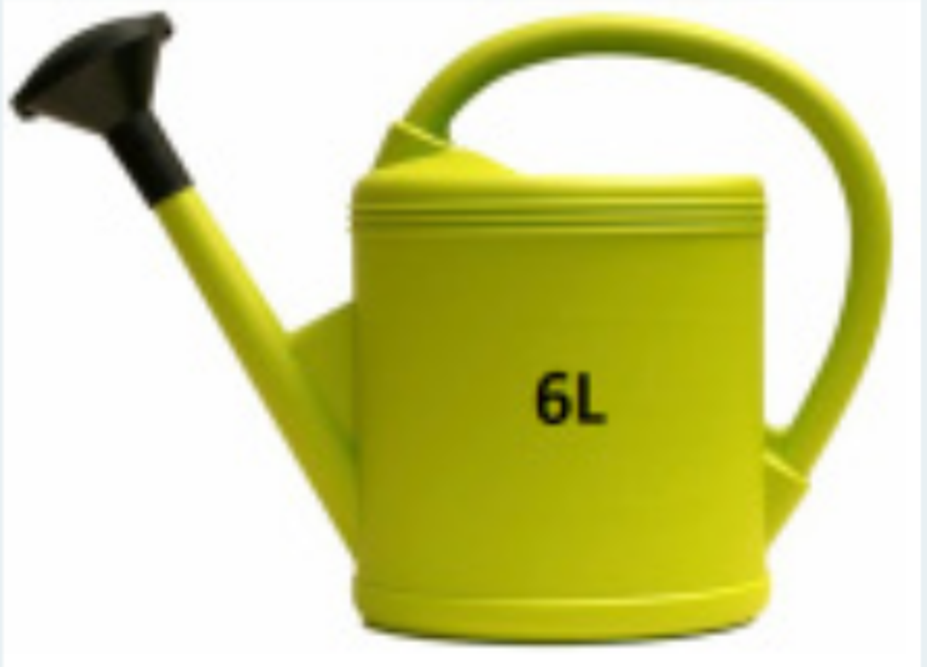
\includegraphics[width=0.8\linewidth]{sources/arrosoir.pdf}
  \end{figure}

\textbf{Combien d’arrosoirs peut-elle remplir si son réservoir d’eau est rempli à 60 \% de sa contenance totale ?}

\textit{On présentera soigneusement toute la démarche suivie.}

On rappelle la formule du volume V d’un cylindre de diamètre D et de hauteur h : $V = \pi \dfrac{D^2}{4}\times h$

\end{multicols}

\newpage

\subsection*{Exercice 2} 

On considère le récipient ci-dessous, obtenu à partir du cône ci-contre que l’on a coupé.

\begin{multicols}{2}

  \begin{figure}[H]
    \centering
    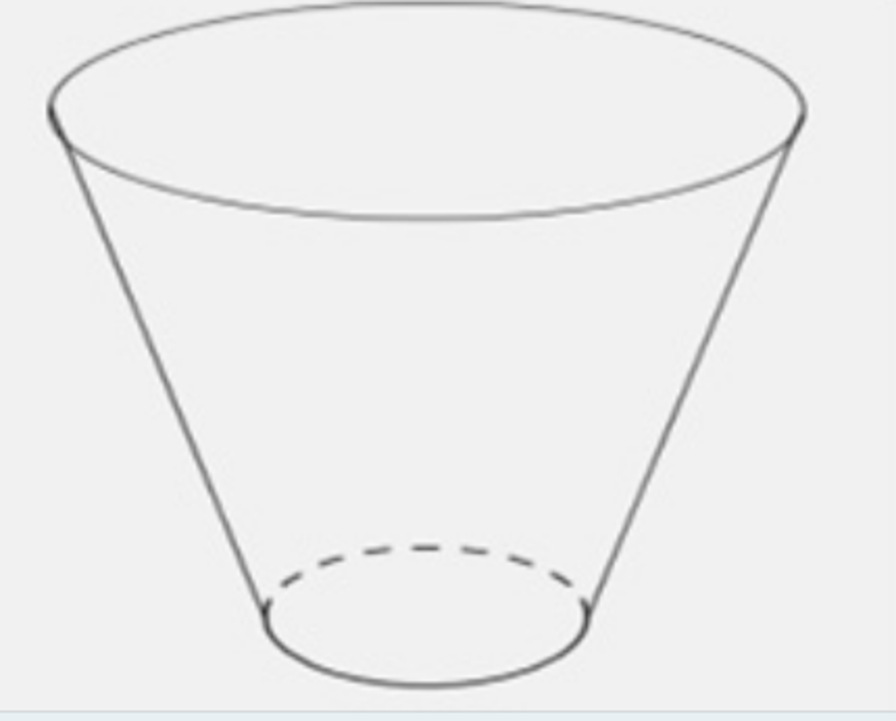
\includegraphics[width=0.8\linewidth]{sources/cone-1.pdf}
  \end{figure}

  \begin{figure}[H]
    \centering
    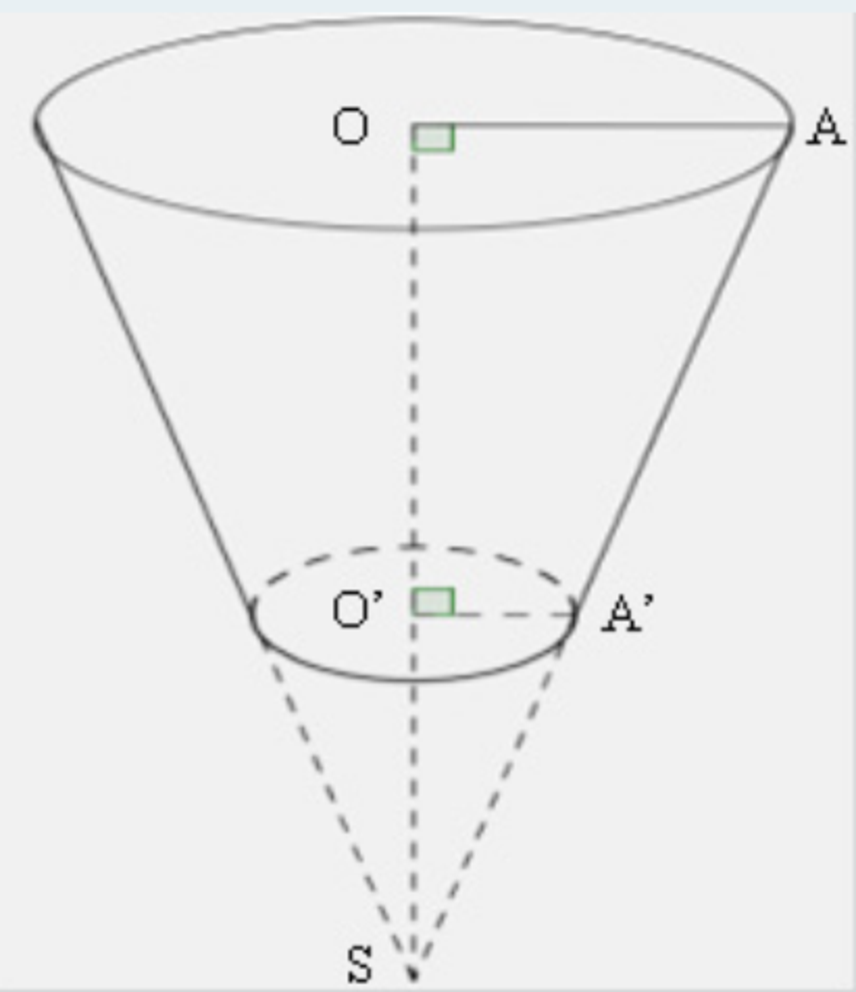
\includegraphics[width=0.8\linewidth]{sources/cone-2.pdf}
  \end{figure}

\end{multicols}

On a : OA = 30 cm ; SO = 50 cm et SO’ = 20 cm.

On remplit ce récipient de sel.

Sachant que la masse volumique du sel est de 2,16 kg/L, calculer la masse du sel contenu dans le récipient ?

On rappelle que le volume d’un cône de révolution est donné par la formule :
$V = \dfrac{\pi R^2 h}{3}$ où R représente le rayon de la base et h la hauteur du cône.

\newpage

\subsection*{Exercice 3}
\begin{multicols}{2}
  \begin{figure}[H]
    \centering
    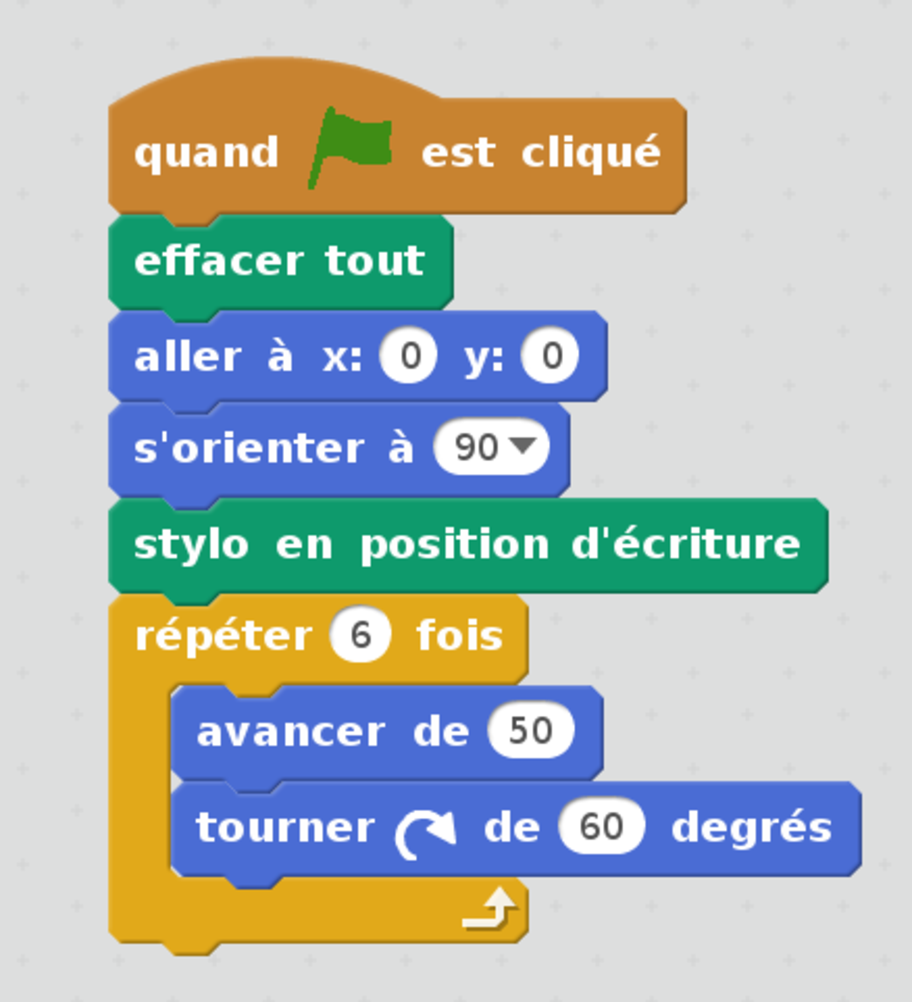
\includegraphics[width=0.8\linewidth]{sources/scratch.pdf}
  \end{figure}

\begin{enumerate}
\item[1.] Reproduire la firgure tracée par le lutin lors de l'execution du script ci-contre.
\item[2.] Écrire un nouveau script afin de tracer un dodécagone régulier. (Polygône avec 12 côtés égaux) 
\end{enumerate}
\end{multicols}
\end{document}
